\documentclass[10pt,spanish,a4paper,openany,notitlepage]{article}
%-------------------------------------Paquetes-----------------------------------------------------------------------
\usepackage[spanish]{babel}  % Traduce los textos a castellano
\usepackage[utf8]{inputenc}	% Permite escribir directamente áéíóúñ
\usepackage{t1enc}            	% Agrega caracteres extendidos al font
\usepackage{amsmath} 		%Permite imprimir mas opcciones matematicas
\usepackage{graphicx}		%Permite agregar imagenes al informe
\usepackage{multicol}  		%Permite dividir el texto en varias columnas
\usepackage{anysize}		%Permite modificar los margenes del documento
\usepackage{float} 			%Permite utilizar H para colocar las imagenes en un lugar especifico 
\usepackage{multirow}		%Permite dividir las tablas en subtablas
\usepackage{booktabs}		%Permiten manejar mejor el tamaño de las tablas
\usepackage{tabulary}		%Permiten manejar mejor el tamaño de las tablas
\usepackage{fancyhdr}		%Permite agregar encabezado y pie fancy
\usepackage{framed}

\usepackage{courier}		%
\usepackage{color}			%
\usepackage{listings}  		%Permite agregar codigo directamente sobre el documento

%---------------------------------------Definiciones propias---------------------------------------------------------
\newcommand{\grad}{\hspace{-2mm}$\phantom{a}^{\circ}$} %El º que no existe como comando
\newcommand{\oiint}{\displaystyle\bigcirc\!\!\!\!\!\!\!\!\int\!\!\!\!\!\int} %Integral doble cerrada
%------------------------------------------------------------------------------------------------------------------------

%-------------------------------------Configuracion De Codigo----------------------------------
\definecolor{dkgreen}{rgb}{0,0.6,0}
\definecolor{gray}{rgb}{0.5,0.5,0.5}

\lstset{language=C,
	breaklines=true,
	keywordstyle=\bf\color{blue},
	commentstyle=\tt\it\color{dkgreen},
	stringstyle=\color{gray},
 	numbers=left,
	numberstyle=\tiny\color{black},
	stepnumber=2,
	numbersep=8pt,
	backgroundcolor=\color{white},
	tabsize=4,
	showspaces=false,
	inputencoding=latin2,
	showstringspaces=false}

\newcommand{\captionlisting}[2][]{%
    \lstinputlisting[caption={\large{\detokenize{#2}}},#1]{#2}%
}

\renewcommand\lstlistingname{Archivo}
%%%%%%%%%%%%%%%%%%%%%%%%%%%%%%%%%%%%%%%%%%%%%%%%%%%

% Título principal del documento.
\title{\textbf{TP1}\\ Generador de fractales Multibrot}

% Información sobre los autores.
\author{Gallipi Leandro, \textit{Padrón Nro. 94274}                    \\
            \texttt{  leandrogallippi@gmail.com }                                              			\\
            Martinez Gaston Alberto, \textit{Padrón Nro. 91383}                     	\\
            \texttt{gaston.martinez.90@gmail.com}                                          			\\[2.5ex]
            \normalsize{Grupo Nro. ? - 2do. Cuatrimestre de 2014}                       	\\
            \normalsize{66.20 Organización de Computadoras - Práctica Martes}  	\\
            \normalsize{Facultad de Ingeniería, Universidad de Buenos Aires}     	\\
       }
\date{}

\begin{document}
\setcounter{page}{0} %De esta manera no se numera la carátula

\maketitle

% Quita el número en la primer página.
\thispagestyle{empty}

% Resumen
\begin{abstract}
El presente trabajo trata sobre el desarrollo de un programa en lenguaje Asembler Mips32 para la generacion de fractales. En el mismo intenta aplicarse conceptos de programacion a bajo nivel tales como el concepto de ABI; o el manejo a nivel procesador de numeros flotantes.
\end{abstract}
 
\newpage

\section{Introducción}

El objetivo del siguiente trabajo práctico es familiarizarse con las instrucciones de MIPS32.  El programa tiene como finalidad generar un archivo en formato PGM para que éste represente el dibujo de un conjunto Multibrot de orden 3 y sus vecindades, en el cual la lógica de cómputo del fractal deberá tener soporte nativo para NetBSD/pmax.\\
Este programa realiza lo mismo que el recibido por la práctica, por lo que el manual y los comandos serán iguales que éstos, y para el usuario será equivalente usar esta implementación o la anterior.

\section{Desarrollo}

\subsection{Recursos y Portabilidad}
En este trabajo se utilizó GXemul para emular la máquina MIPS32. A continuación, se dejan expresados los comandos que se utilizaron para transmitir los archivos al emulador.\\
La transferencia de archivos entre la máquina host y la guest se hizo mediante SSH. Se procedió de la siguiente manera:\\
\begin{itemize}
\item[*] Para trabajar con el GXemul se procedió primero creando una nueva interfaz de red (debe crearse cada vez que se inicia el host y con permisos de administrador):
\item[-]\texttt{hostOS\$ sudo ifconfig lo:0 172.20.0.1}
\item[*] Luego se ejecuto el GXemul en modo X:
\item[-]\texttt{hostOS\$ ./xgxemul -e 3max -d netbsd-pmax.img -x}
\item[*] Una vez ya ingresado con el usuario y la contraseña en la máquina simulada, se creó un túnel reverso para saltear las limitaciones propias del GXemul:
\item[-]\texttt{guestOS\$ ssh -R 2222:127.0.0.1:22 usuario@172.20.0.1}
\item[*] A partir de ese momento y dejando lo anterior en segundo plano, ya se puede trabajar mediante SSH de manera más cómoda:
\item[-]\texttt{hostOS\$ ssh -p 2222 root@127.0.0.1}
\end{itemize}
\subsection{Diseño del algoritmo}
El algoritmo original provisto por la cátedra es de la forma:
\begin{framed}
\begin{verbatim}para cada pixel $p {
    $f = $c = complejo asociado a $p;
        for ($i = 0; $i < $N - 1; ++$i) {
            if (abs($f) > 2)
                break;
            $f = $f * $f * $f + $c;
        }
        dibujar el punto p con brillo $i;
}\end{verbatim}
\end{framed}

\subsection{Implementación}
Se dividio entonces el codigo en las siguientes partes principales:

\begin{itemize}
\item print\_header: Imprime el header del pgm. Si bien se pudo haber realizado de manera mucho mas generica, se opto por una forma un poco mas funcional y hardcodeada.
\item plot\_loop\_y: Ciclo principal, recorre los puntos segun su coordenada y
\item plot\_loop\_X: Ciclo secundario, recorre los puntos segun su coordenada x, y se ejecuta completo una vez por cada ciclo `y'
\item shining\_loop: Aqui se realiza el calculo del brillo de cada pixel.
\item print\_shining: Imprime el brillo de cada pixel calculado en el ciclo anterior. Al igual que con la impresion del header, se opto por una solucion mucho mas hardcodeada y funcional que por una version generica.
\end{itemize}

A saber: Los ciclos utilizan los registros \$t8 y \$t9 como contadores. Por alguna razon que no llegamos a descubrir, el contenido de los mismos no se llegaba a mantener constante durante la ejecucion del ciclo y generaba un ciclo infinito en la entrega original. Esto no es reproducible si se ejecuta el programa \textit{step by step} con el GDB. Se opto como solucion, guardar el contenido de los registros en la LTA para preservar su valor. Esto si bien genera mucha mas carga, inicialmente inecesaria, soluciono el problema.


\subsection{Salida: Formato PGM}

La salida del programa se da mediante un formato conocido como \textit{Portable GrayMap} o "\textit{PGM}". El mismo admite dos versiones, binaria y ascii. Se opto por la salida ascii para el guardado de archivos, ya que de esta
forma, no habria que modificar nada mas que el archivo de salida si se decide mostrar el resultado por STDOUT.\\
Asi mismo, el formato \textit{PGM} concede varias libertades: siempre que se respete el siguiente orden, la salida ascii podra estar organizada en una o mas lineas:

\[ <tipo> <ancho> <alto> <intensidad> (0,0) (1,0) ... (X,0) (0,1) ... (Y,X)  \] 

En nuestro caso, optamos por el siguiente estandar:

\begin{framed}
\begin{verbatim}<tipo>
<ancho>
<alto>
<intensidad>
[(0,0),(1,0),...,(X,0),(0,1),(1,1),...,(X,1),...,(0,Y),(1,Y),...,(X,Y)]
\end{verbatim}
\end{framed}

Ademas, por un tema de simplicidad, se tomo un largo arbitrario en la longitud de los numeros considerando que:
\begin{itemize}
\item Las dimensiones de una pantalla poseen a lo sumo 4 digitos.
\item El brillo de cada pixel posee a lo sumo un largo 3, dado que son valores comprendidos entre 0 y 255. 
\end{itemize}
Ejemplo:
\begin{framed}
\begin{verbatim}P2
0004
0002
006
000 001 005 003 002 006 006 004\end{verbatim}
\end{framed}

\section{Compilacion}
Para compilar el trabajo práctico, se tienen que ejecutar las siguientes líneas en la terminal de NetBSD, habiendo pasado previamente los archivos.\
\texttt{gcc -Wall -O -c main.c}
\texttt{gcc -c mips32\_plot.S}
\texttt{gcc -o tp1 main.o mips32\_plot.o}
Para simplificar este proceso, y no tener que escribir el comando entero, se modifico el Makefile original provisto por la catedra, mediante el cual, con solo escribir 'make', se compila el trabajo práctico.

\begin{framed}
\begin{verbatim} $make\end{verbatim}
\end{framed}

Ademas, se provee de un comando para la limpieza de los archivos extras y el ejecutable. El mismo se ejecuta mediante el comando:

\begin{framed}
\begin{verbatim}    $ make clean\end{verbatim}
\end{framed}

\section{Ejecuciones de prueba}

\begin{enumerate}
\item Se corre el programa para las coordenadas complejas 0+0i con una resolución de 1x1:   ./tp1-2014-2-bin --center 0+0i --resolution 1x1 -o test1-tp.pgm 
\begin{figure}[hbt]
\centering

\includegraphics[width=0.25\textwidth]{test1-tp.jpg}
\caption{Prueba 1}
\end{figure}
\item Se corre el programa centrandolo ahora en un punto que seguro no pertenecen al conjunto:  ./tp1-2014-2-bin -c 10+0i -r 1x1 -o test2-tp.pgm
\begin{figure}[hbt]
\centering

\includegraphics[width=0.25\textwidth]{test2-tp.jpg}
\caption{Prueba 2}
\end{figure}
\item Ejemplo donde no se ejecuta correctamente el programa:  ./tp1-2014-2-bin -r 1X1 -w 0.0001 -o test3-tp.pgm 
\begin{framed}
\begin{verbatim}Usage: 
  ./tp1-2014-2-bin -h 
  ./tp1-2014-2-bin -V 
  ./tp1-2014-2-bin [options] 
Options: 
  -r, --resolution  Set bitmap resolution to WxH pixels. 
  -c, --center      Set coordinates for the center of the image. 
  -w, --width       Change the width of the spanned region. 
  -H, --height      Change the height of the spanned region. 
  -o, --output      Path to output file. 
Examples: 
  ./tp1-2014-2-bin -o output.pgm 
  ./tp1-2014-2-bin -r 1600x1200 -o output.pgm 
  ./tp1-2014-2-bin -c +0.282+0.01i -o output.pgm \end{verbatim}
\end{framed}
\item. Se corre el programa usando los valores por defecto, barriendo la región rectangular del plano comprendida entre los vértices -0.65 + 0.30i y -0.55 + 0.20i:  ./tp1-2014-2-bin -o test4-tp.pgm
\begin{figure}[hbt]
\centering
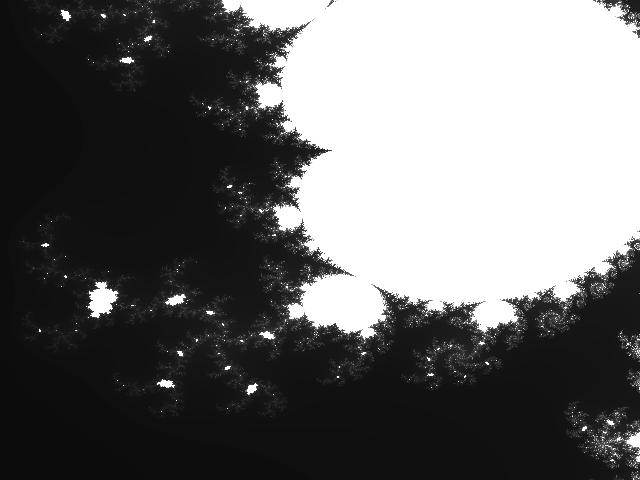
\includegraphics[width=0.25\textwidth]{test4-tp.jpg}
\caption{Prueba 4}
\end{figure}
\item Hacemos zoom sobre la región centrada en -0.6 + 0.6i, usando un rectángulo de 0.05 unidades de lado:  ./tp1-2014-2-bin --center -0.6+0.6i --width 0.05 --height 0.05 -o test5-tp.pgm
\begin{figure}[hbt]
\centering
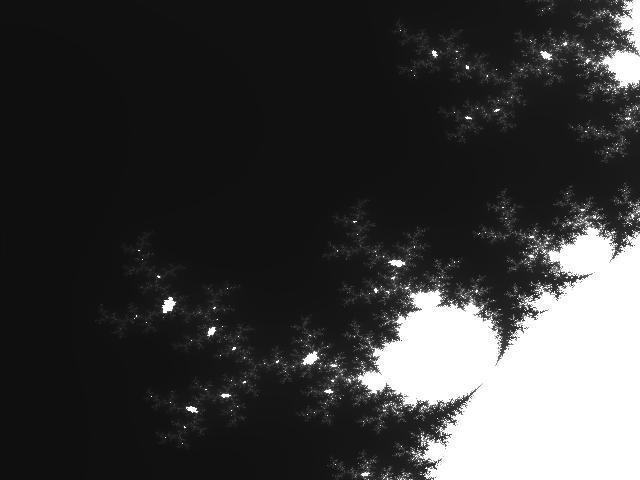
\includegraphics[width=0.25\textwidth]{test5-tp.jpg}
\caption{Prueba 5}
\end{figure}
\end{enumerate}

\section{Conclusiones}

En el trabajo práctico se pudo aprender no solo las instrucciones necesarias para poder trabajar en Assembler MIPS 32, sino la forma de organizarlo y diseñarlo. Esto es de suma importancia, no solo para la aprobación de esta materia, sino para poder entender cómo se trabaja en niveles computacionales muy bajos.\\
Además, dada la necesidad de debugear el programa, se aprendió mucho sobre el manejo de GDB.
\newpage
\appendix
\section{Codigo Mips}

\captionlisting{mips32_plot.S}

\newpage
\section{Makefile}

\lstinputlisting[language=make,
			breaklines=true,
			keywordstyle=\bf\color{blue},
			commentstyle=\tt\it\color{dkgreen},
			stringstyle=\color{gray},
 			numbers=left,
			numberstyle=\tiny\color{black},
			stepnumber=1,
			numbersep=8pt,
			backgroundcolor=\color{white},
			tabsize=4,
			showspaces=false,
			showstringspaces=false]{Makefile.in}

\newpage
% Citas bibliográficas.
%\begin{thebibliography}{99} %Hasta 99 

%\bibitem{?}

%\end{thebibliography}

\end{document}
